\chapter{Solution Techniques\label{cha:chapter3}}
The solution of the PDEs may not be trivial. Hence, numerical techniques are employed to find an approximate solution for the given PDE. Our choice for the numerical solution is FEM (Finite Element Method) because of its versatility in dealing with complex boundaries.
The FEM technique focuses on dividing the problem into smaller subdomains while approximating the solution within each subdomain using the interpolation functions and assembling the element equation into a global system to ultimately solve the resulting system of equations while incorporating boundary conditions. 

\section{Enthalpy Problem\label{sec:reqoverview}}

In FEM simulations, one of the most popular weighted residual methods is Galerkin's method\cite{galerkin1915series}. Boris Grigoryevich Galerkin pioneered the method in the year 1915\cite{galerkin1915series}. He found that the approximation is determined from the condition that the residual is orthogonal to a system of linearly independent test functions and the orthogonality is understood in the integral sense\cite{Repin+2017+351+357}. We employ his method in our FEM solution to find the approximate solution of the forms $\tilde{H}(z,t) = \sum_{i=0}^NH_i(t)\phi_i(z) \; \text{and}\; \tilde{T}(z,t) = \sum_{i=0}^NT_i(t)\phi_i(z)$.\\  Where, $\phi_i(z)$ is defined as the hat function.\\
While keeping the time = t, we divide our domain $0 \leq z \leq z_b$into N sub intervals \cite{verhoeven2003modelling}.\\The matrix representation of our  variational form \eqref{eq:Entalpyvarform}  is as below\cite{verhoeven2003modelling}.
\begin{subequations}
\begin{align}
    \underline{\mathbf{M}}\frac{d\underline{\mathbf{H}}}{dt} = D\underline{\mathbf{b}}-D\underline{\mathbf{N}}\underline{\mathbf{T}} \label{eq:discretEnthlp}
\end{align}
\end{subequations}

\subsection{Time integration methods\label{sec:overviewsuba}}
The variables that are dependent on time (for example in our case the enthalpy is a time dependent variable $\Dot{H}$), Euler backward (or Euler implicit) scheme \cite{butcher2016numerical} is employed for time integration scheme as it is relatively stable for a larger step size \cite{Stuart:2022}. Hence, the equation \eqref{eq:discretEnthlp} can be rewritten as follows: -\\
\begin{subequations}
\begin{align}
&\underline{\mathbf{H}}^{k+1,l} = \underline{\mathbf{H}}^{k+1,l-1} - (\partial{\underline{\mathbf{G}}(\underline{\mathbf{H}}^{k+1,l-1})}^{-1}\underline{\mathbf{G}}(\underline{\mathbf{H}}^{k+1,l-1})) \\
&\text{Where, $l$ = newton raphson step} \nonumber
\end{align}
\end{subequations}
\begin{subequations}
\begin{align}
&M_{ij} = \int_0^{zb} \phi_i \phi_j dz,\quad \quad N_{ij} = \int_0^{zb} \frac{d\phi_i}{dz}\frac{d\phi_j}{dz}  dz \label{eq:Descritized_form_mass_matrix}
\end{align}
\end{subequations}
\begin{subequations}
\begin{align}
&b_j = \frac{I}{I_{ref}}\phi_j(0)-T_a\int_0^{zb}\frac{d\phi_N}{dz}\frac{d\phi_j}{dz}  dz \label{eq:Descritised_b_matrix}
\end{align}
\end{subequations}
\begin{subequations}
\begin{align}
&\underline{\mathbf{G}}(\underline{\mathbf{H}}^{k+1}) = \underline{\mathbf{M}}(\underline{\mathbf{H}}^{k+1} - \underline{\mathbf{H}}^{k}) - \Delta t(\mathcal{F}(\underline{\mathbf{H}}^{k+1}, t^{k+1})) \label{eq:Descritised_G_matrix}
\end{align}
\end{subequations}
\begin{subequations}
\begin{align}
&\mathcal{F}(H,t) = D(\underline{\mathbf{b}}(t)-\underline{\mathbf{N}}\underline{\mathbf{T}}(\underline{\mathbf{H}})).
\end{align}
\end{subequations}
\begin{subequations}
\begin{align}
&\partial \underline{\mathbf{G}}(\underline{\mathbf{H}}) = \underline{\mathbf{M}}+\Delta t D \underline{\mathbf{N}} \frac{\partial{\underline{\mathbf{T}}}}{\partial{\underline{\mathbf{H}}}}(\underline{\mathbf{H}}) \label{eq:Decretized_dG_matrix}
\end{align}
\end{subequations}
The equations \ref{eq:Descritized_form_mass_matrix} and \ref{eq:Descritised_b_matrix} are programmed in the material subroutine along with $\frac{\partial \underline{\mathbf{T}}}{\partial \underline{\mathbf{H}}}(\underline{\mathbf{H}})$ and equations \ref{eq:Descritised_G_matrix} to \ref{eq:Decretized_dG_matrix} are programmed in element subroutine.\\ \\
Our problem will be solved as per the algorithms given in section \ref{sec:Flowcharts} along with the suitable initial conditions discussed in the section \ref{sec:initial_condition_given}.
\section{Stefan Problem\label{sec:Stefan_solution}}
We again use the Galerkin's method\cite{galerkin1915series} in the formulation of our FEM scheme.
We divide the domains $0 \leq z \leq s(t)$ and $s(t) \leq z \leq z_b$ into $N$ and $M$ equal sub intervals respectively. We find the approximate solution of the forms
\begin{subequations}
    \begin{align}
        T_{h_l}(z,t) = \sum_{j = 0}^{N} T_{l,j}(t)\phi_{l,j}(z,t), \quad\quad T_{h_s}(z,t) = \sum_{j=0}^M T_s,j(t)\phi_{s,j}(z,t).
    \end{align}
\end{subequations}
Incorporating the boundary conditions as $T_{l,N}(t) = 0$ and $T_{s,M}(t) = T_a$, we ensure the fulfillment of Dirichlet condition. Substituting the above approximations in the weak form \eqref{eq:Stefan_Weak_formorig} and \eqref{eq:Stefan_Weak_formcalc} yields the two system of equations in the matrix form 
\begin{subequations}
    \begin{align}
        &\underline{\mathbf{M_l}}\frac{d \underline{\mathbf{T_l}}}{dt} + \underline{\mathbf{N_l}}\underline{\mathbf{T_l}} = \underline{\mathbf{b_l}} \label{eq:descretised_stefan1},\\
        \nonumber \\
        &\underline{\mathbf{M_s}}\frac{d \underline{\mathbf{T_s}}}{dt} + \underline{\mathbf{N_s}}\underline{\mathbf{T_s}} = \underline{\mathbf{b_s}} \label{eq:Descritised_stefan2}
    \end{align}
\end{subequations}

\subsection{Time integration methods\label{sec:Stefan_time_integration}}
We employ the Crank-Nicolson scheme for the time integration of the temperature distribution evaluation which is \textit{O}($\Delta t^2$) and Euler Forward scheme for evaluating the position of the solid liquid interface. We now describe each term in the equations \ref{eq:descretised_stefan1} and \ref{eq:Descritised_stefan2} which are coded in our element subroutine of the Stefan Problem Approach.
\begin{subequations}
    \begin{align}
        &M_{l,0 \ 0} = \frac{1}{2}h_l(t), \quad \quad M_{l,i \ i} = h_l(t) \quad i = 1,\ldots,N-1,\label{eq:Stefan_material1}\\
        \nonumber \\
        &N_{l,i-1 \ i} = -\frac{1}{6}\frac{3i-2}{N}\frac{ds}{dt} - \frac{1}{h_l(t)}, \quad \quad N_{l,i+1 \ i} = \frac{1}{6}\frac{3i+2}{N}\frac{ds}{dt} - \frac{1}{h_l(t)}, \\
        \nonumber \\
        &N_{l,0 \ 0} = \frac{1}{6N}\frac{ds}{dt} + \frac{1}{h_l(t)}, \quad \quad N_{l,i \ i} = \frac{1}{3N}\frac{ds}{dt} + \frac{2}{h_l(t)}, \quad \quad i = 1,\ldots,N-1,\\
        \nonumber \\
        &b_{l,0} = \frac{I}{I_{ref}},\\
        \nonumber \\
        &M_{s,i \ i} = h_s(t), \quad \quad \quad b_{s,M-1} = T_a \left( \frac{1}{3} \frac{ds}{dt} + \frac{1}{h_s(t)} \right),\\
        \nonumber \\
        &N_{s,i-1 \ i} = -\frac{1}{6} \frac{3M-3i+2}{M} \frac{ds}{dt} - \frac{1}{h_s(t)}, \quad N_{s,i+1 \ i} = \frac{1}{6} \frac{3M-3i-2}{M} \frac{ds}{dt} - \frac{1}{h_s(t)},\\
        \nonumber \\
        &N_{s,i \ i} = -\frac{1}{3M} \frac{ds}{dt} + \frac{2}{h_s(t)}.\label{eq:Stefan_material2}
        \end{align}
\end{subequations}
The position of the interface can be calculated from the Stefan Condition \ref{eq:Stefan_specialBc}, which is discretized as below
\begin{subequations}
    \begin{align}       
        &s^{k+1} = s^{k} + \frac{\Delta t}{\lambda_f}\left \{ \frac{1}{h_l(t^k)}T_{l,N-1}^k + \frac{1}{h_s(t^k)}T_{s,1}^k \right \}
        \end{align}
\end{subequations}
Using the Crank-Nicolson scheme, we find the temperature distribution for the next time step in both the phases as follows
\begin{subequations}
    \begin{align}
        \begin{split}
            &\left(\underline{\mathbf{I}} + \frac{1}{2}\Delta t (\underline{\mathbf{M}}_l^{k+1})^{-1}\underline{\mathbf{N}}^{k+1}_l \right)\underline{\mathbf{T}}^{k+1}_l = \left(\underline{\mathbf{I}} - \frac{1}{2}\Delta t (\underline{\mathbf{M}}_l^{k})^{-1}\underline{\mathbf{N}}^{k}_l \right)\underline{\mathbf{T}}^{k}_l +\\
            &\hspace{6cm} \Delta t\left(\frac{1}{2}(\underline{\mathbf{M}}_l^{k+1})^{-1} + \frac{1}{2}(\underline{\mathbf{M}}_l^{k})^{-1} \right)\underline{\mathbf{b}}_l
        \end{split}
        \end{align}
\end{subequations}
and,
\newpage
\begin{subequations}
    \begin{align}
        \begin{split}
            & \left(\underline{\mathbf{I}} + \frac{1}{2}\Delta t (\underline{\mathbf{M}}_s^{k+1})^{-1}\underline{\mathbf{N}}^{k+1}_s \right)\underline{\mathbf{T}}^{k+1}_s = \left(\underline{\mathbf{I}} - \frac{1}{2}\Delta t (\underline{\mathbf{M}}_s^{k})^{-1}\underline{\mathbf{N}}^{k}_s \right)\underline{\mathbf{T}}^{k}_s +\\
            & \hspace{6cm} \Delta t\left(\frac{1}{2}(\underline{\mathbf{M}}_s^{k+1})^{-1}\underline{\mathbf{b}}_s^{k+1} + \frac{1}{2}(\underline{\mathbf{M}}_l^{k})^{-1}\underline{\mathbf{b}}_s^k \right)\\
        \end{split}
    \end{align}
\end{subequations}

In the next section we discuss the derivation of the inital conditions.


\section{Initial Conditions \label{sec:initial_condition_given}}
For both the the schemes described above, we need a suitable initial condition. During the premelting stage the temperature in the material is governed by the heat equation \eqref{eq:Heat_equation}.
\begin{subequations}
    \begin{align}
        \frac{\partial T}{\partial t} = \frac{\partial^2 T}{\partial z^2} \label{eq:Heat_equation}\\ 
        \nonumber
        \end{align}
\end{subequations}
Assuming the following initial and boundary conditions. \\
The (dimensionless) energy supplied at the surface which is denoted by F. \\
\begin{subequations}
    \begin{align}
        \frac{\partial T}{\partial z} = -F, \quad z = 0 \\ \nonumber
    \end{align}
\end{subequations}
Subject to the boundary condition: \\
\begin{subequations}
    \begin{align}
        T \rightarrow T_a, \quad z \rightarrow \infty
        \end{align}
\end{subequations}
Initially we assume: \\
\begin{subequations}
    \begin{align}
        T = T_a, \quad t = 0 \label{eq:Initial_condition}
        \end{align}
\end{subequations}
The solution to the equations \eqref{eq:Heat_equation} to \eqref{eq:Initial_condition} has been founded by using Laplace Transform by \cite{verhoeven2003modelling} in his paper
\begin{subequations}
    \begin{align}
    T(z,t) = F \left\{ 2 \left(\frac{t}{\pi} \right)^{\frac{1}{2}} \exp\left(-\frac{z^2}{4t}\right)-z \operatorname{erfc}\left(\frac{z}{2t^{\frac{1}{2}}}\right) \right\} + T_a \label{eq:Initial_Temp_Distribution}
    \end{align}
\end{subequations}
Using equation \eqref{eq:Initial_Temp_Distribution} we find the initial temperature distribution in the material .\\

Since, for the Stefan Problem we assume some part of the material is already melted, we need an initial temperature distribution in the liquid  as well as the solid phase of the material. The equation \eqref{eq:Inital temp in the liquid} gives the initial temperature distribution in the liquid domain, satisfying the boundary condition at $z = s$ in the liquid domain. Where as, the equation \ref{eq:Solid domain temperature} along with the equation \ref{eq:named F} gives the initial temperature distribution in the solid domain  that satisfy the boundary condition at $z = s$ and $z = z_b$  in the solid domain.\\
\begin{subequations}
    \begin{align}
        &T_{l,j}(\Delta t) = \frac{I}{I_{ref}}(s-z_{l,j}), \quad \quad j=0,\ldots,N-1 \label{eq:Inital temp in the liquid} \\
        \begin{split}
        &T_{s,j}(\Delta t) = |T_a|\exp\left(-\frac{(z_{s,j}-s)^2 F^2}{T_a^2 \pi}\right)-F(z_{s,j}-s)\operatorname{erfc}\left(\frac{(z_{s,j}-s)F}{|T_a|\sqrt{\pi}}\right) + T_a,\label{eq:Solid domain temperature}\\
        &\hspace{10cm} j = 1,\ldots,M-1 
        \end{split}\\
        \nonumber \text{Where,}\\
        &F = \frac{I}{I_{ref}}-\lambda_f \frac{ds}{dt}\label{eq:named F}.        
    \end{align}\\
    \nonumber \text{}\\ 
    
\end{subequations}

\section{Flow Charts\label{sec:Flowcharts}}
We have used the Object Oriented Programming (OOP) to program both the schemes. The advantage of OOP is that it offers a combination of data (attributes) and functions (Methods) in a single unit known as class as shown in figure \ref{fig:Structure_of_class}. A class is a blue print that facilitates instructions to create an object. An object in simple terms is a collection of attributes and methods. Methods control the behaviour of these attributes. A class is called child class when it inherits (acquires) the attributes and methods form another class. The class from which the attributes and methods are inherited is referred to as parent class. The advantage this method of programming is that, when we pass an object, a collection of attributes and methods is passed simultaneously making it easier to keep a track of variables, and the role and scope of each class is clearly defined from its attributes and methods.\\
An overview of the enthalpy problem approach program is given in the following flow charts. The flow chart for the material model for the enthalpy problem approach is not provided as the equations \eqref{eq:Descritized_form_mass_matrix} to \eqref{eq:Decretized_dG_matrix} are programmed in the material model for the enthalpy problem and element subroutine is not provided for the Stefan problem approach and equations \ref{eq:Stefan_material1} to \ref{eq:Stefan_material2} are programmed directly in the element subroutine, eliminating the need of the shape functions. Also, the processed inputs, variable updater and post processors are not shown here as they perform non dimensionalization of the variables or plotting graphs. The variable updater is a program which converts the enthalpy to temperature and vice versa according to the material type. Also, the flow charts all the attributes are bold to show they are scalar, and the attributes in bold and with an underline represent vector or matrix. Methods are not represented here with an underline or in bold.\\ 
\begin{figure}[htb]
  \centering
  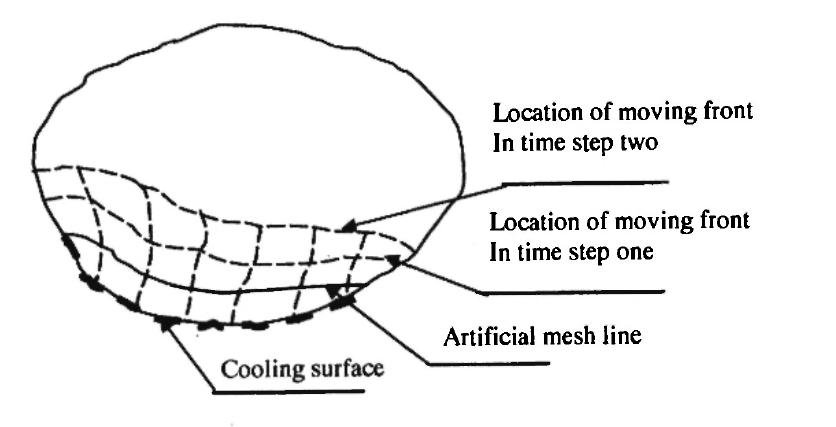
\includegraphics[width=5cm]{img/Newstefanproblemakjfjk.png}\\
  \caption{The mesh generation in Stefan problem 2D. (Figure taken from \cite{Wu+2005+281+288}}
  \label{fig:New mesh generation}
\end{figure}
\begin{figure}[htb]
  \centering
  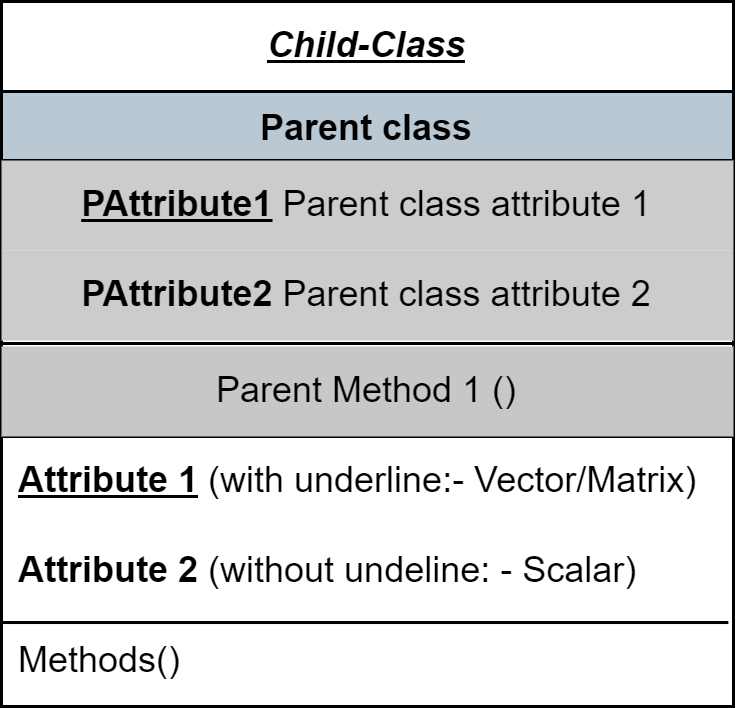
\includegraphics[width=5cm]{img/Nomenclature_Class.png}\\
  \caption{Structure of Class}
  \label{fig:Structure_of_class}
\end{figure}

\begin{figure}[htb]
  \centering
  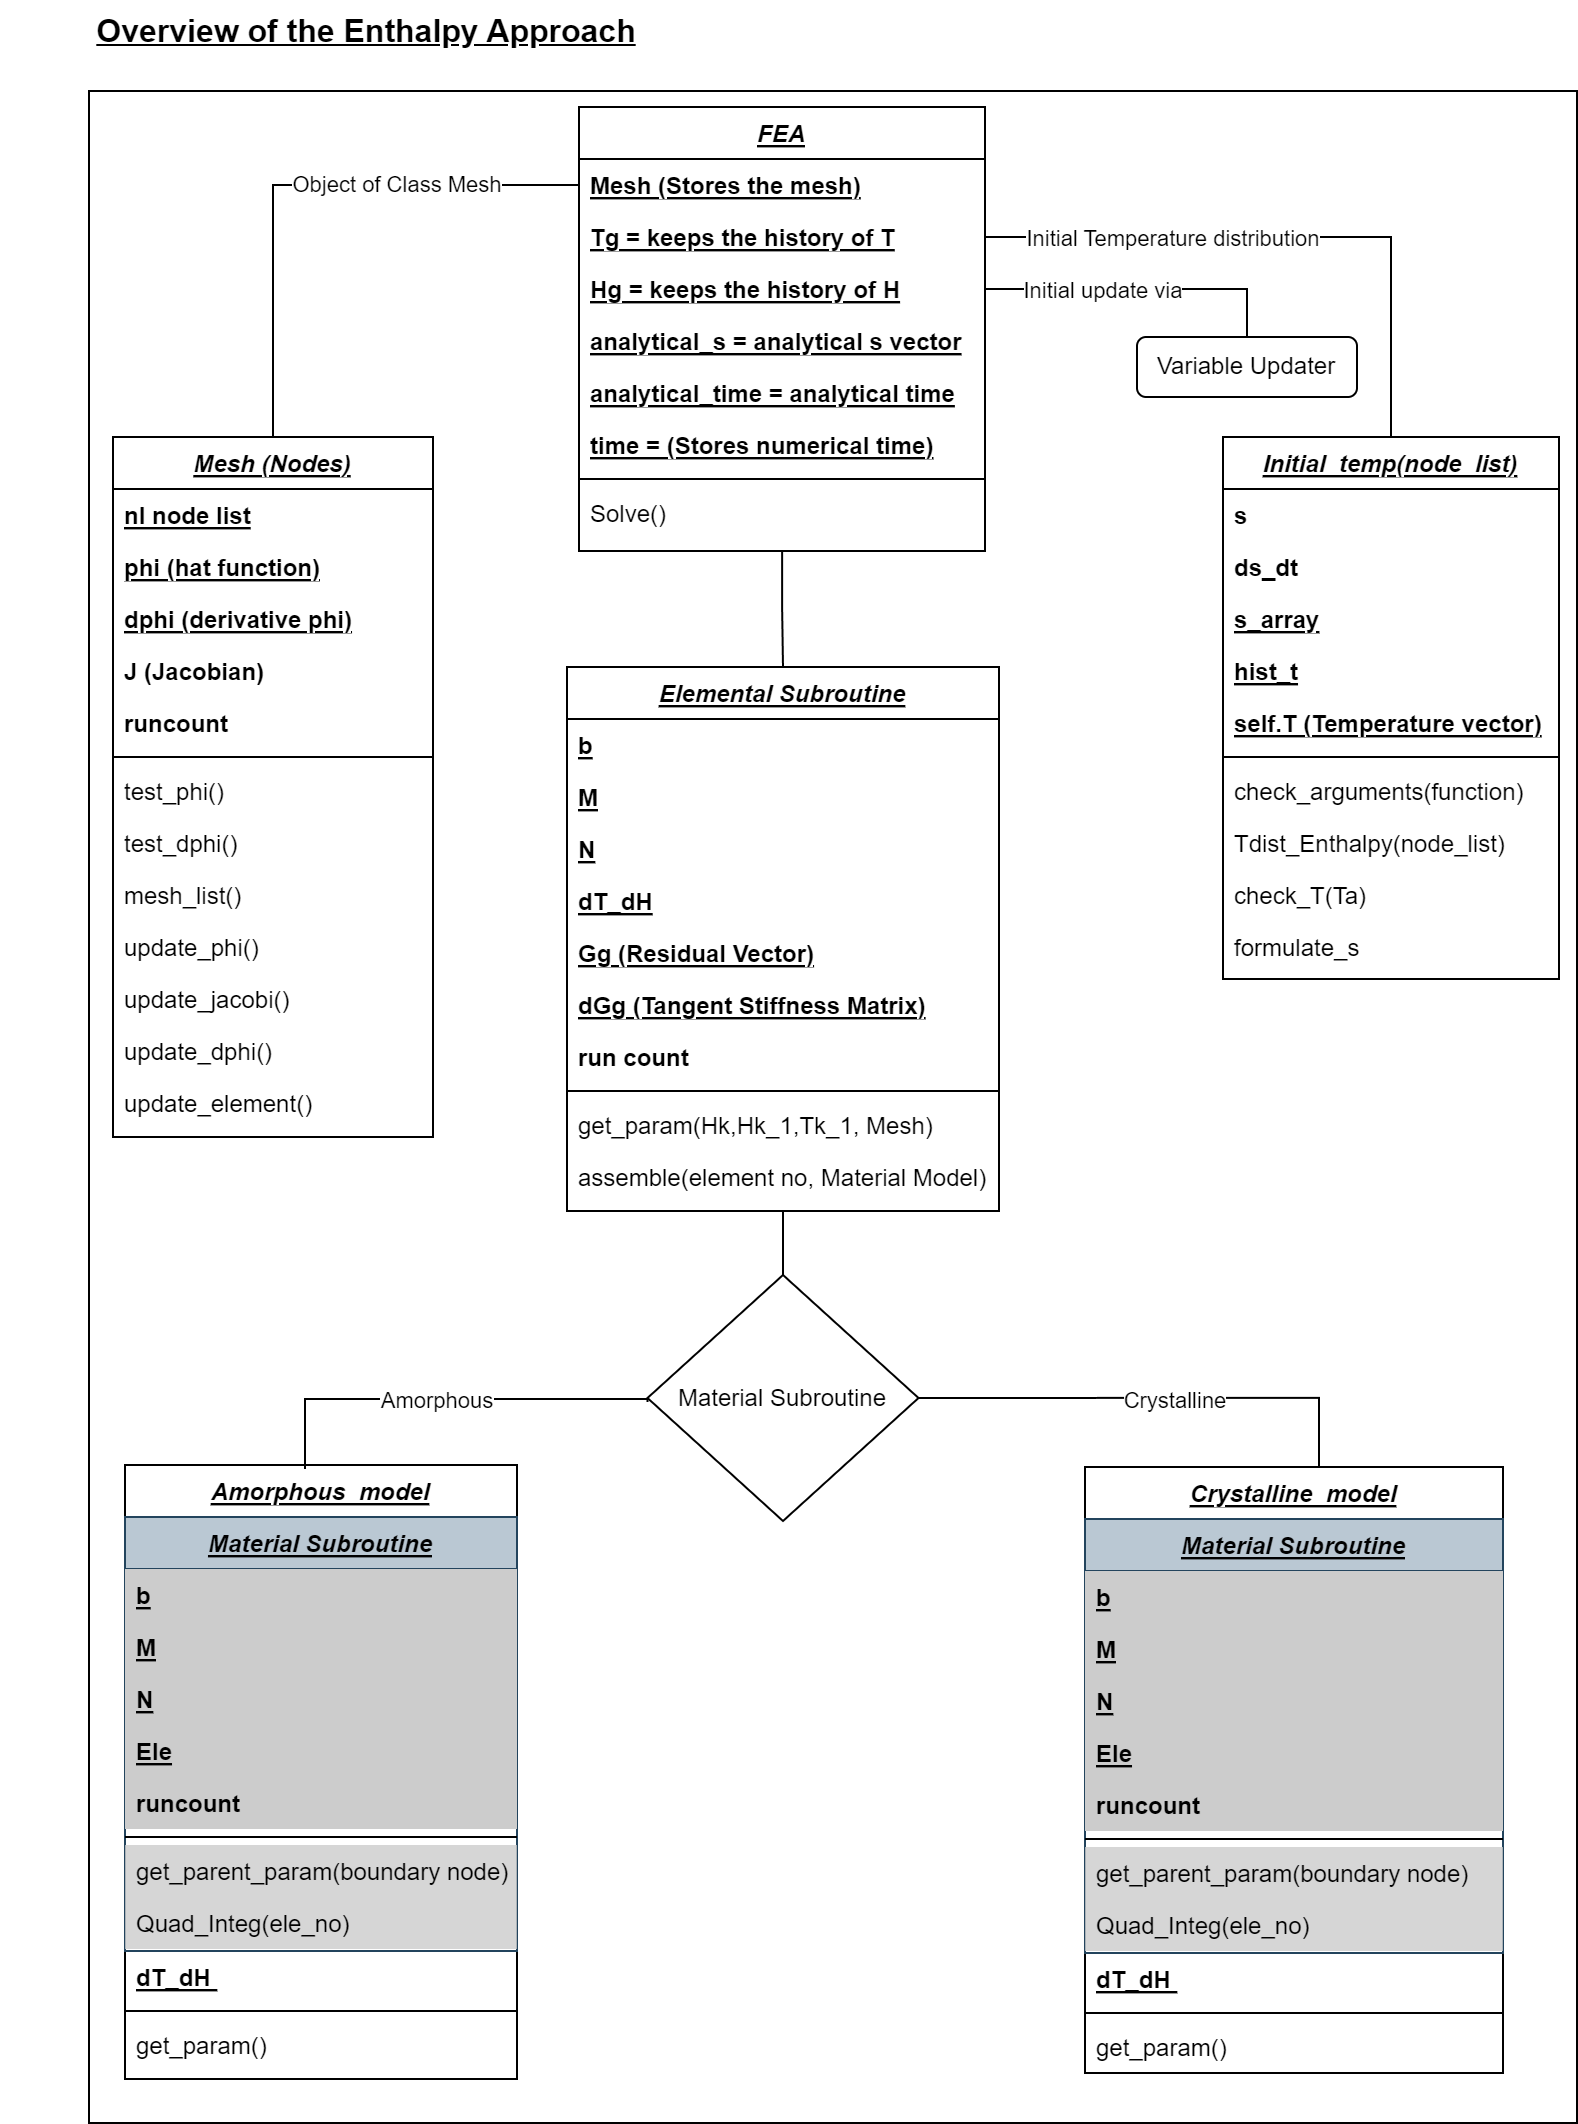
\includegraphics[width=14.3cm]{img/Over_View.png}\\
  \caption{Overview of the Enthalpy Problem Approach}
  \label{fig:Initial_temp}
\end{figure}

\begin{figure}[htb]
  \centering
  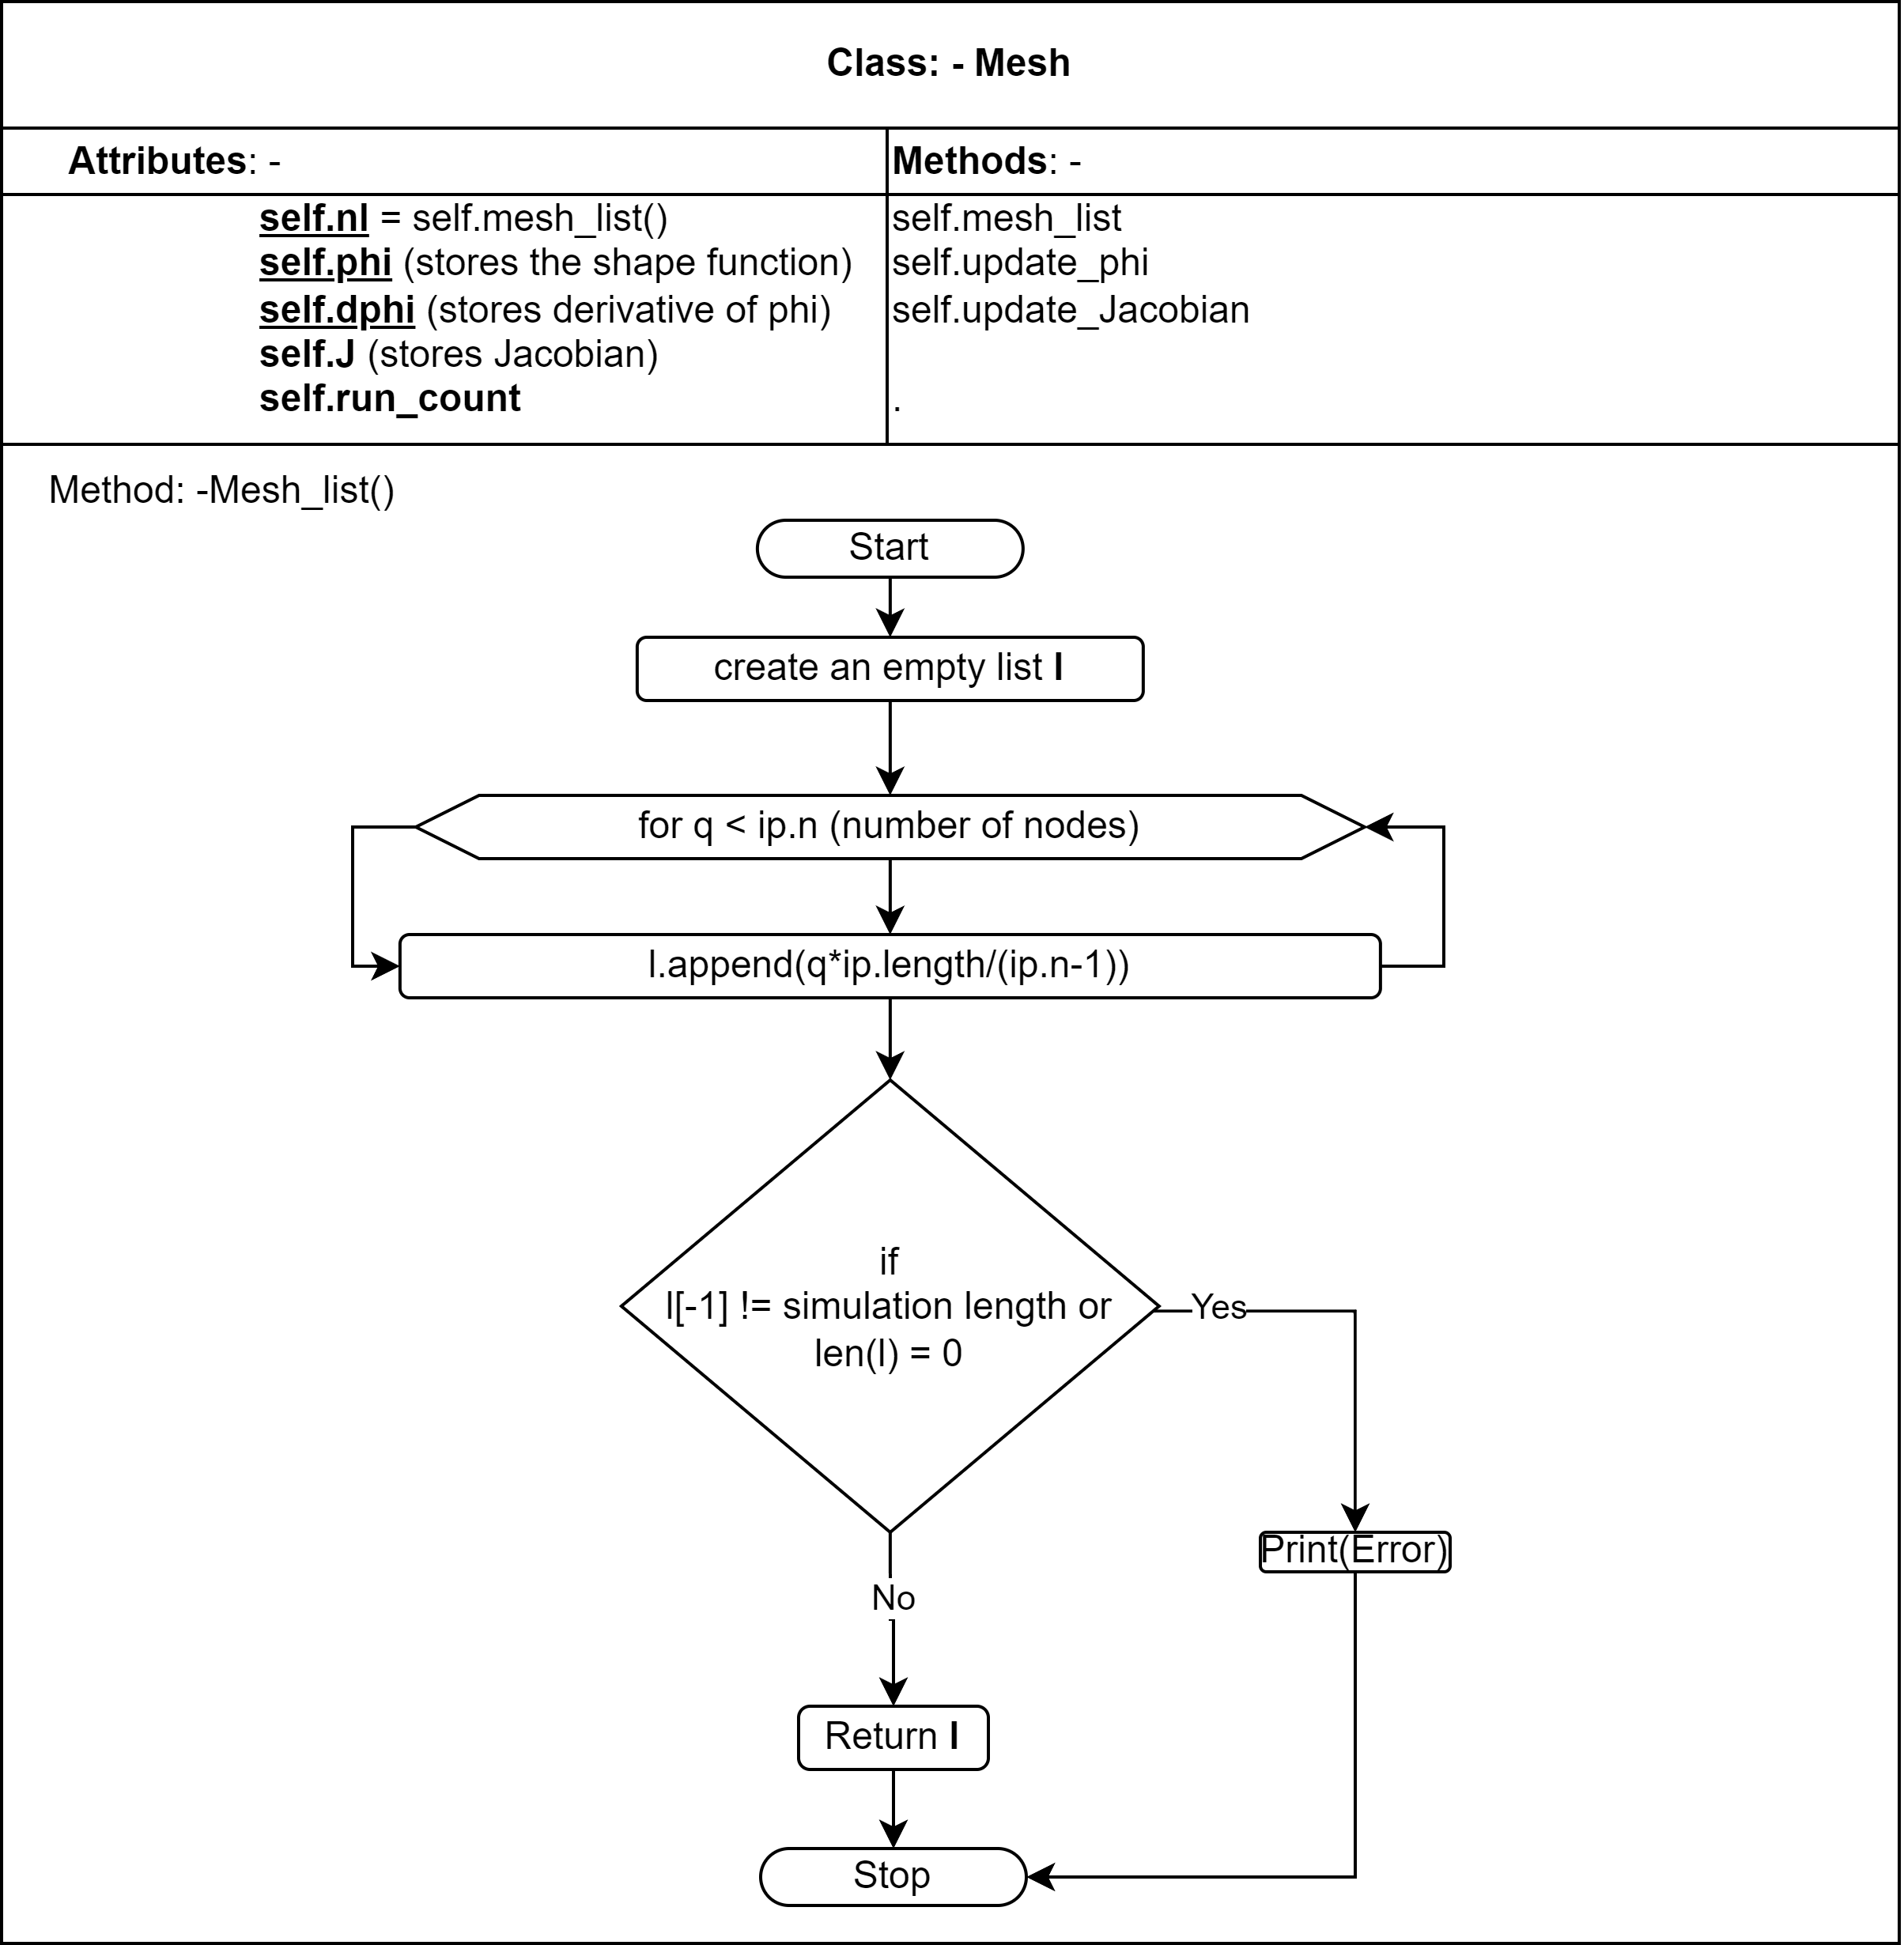
\includegraphics[width=13cm]{img/Mesh.png}\\
  \caption{Mesh}
  \label{fig:Mesh}
\end{figure}

\begin{figure}[htb]
  \centering
  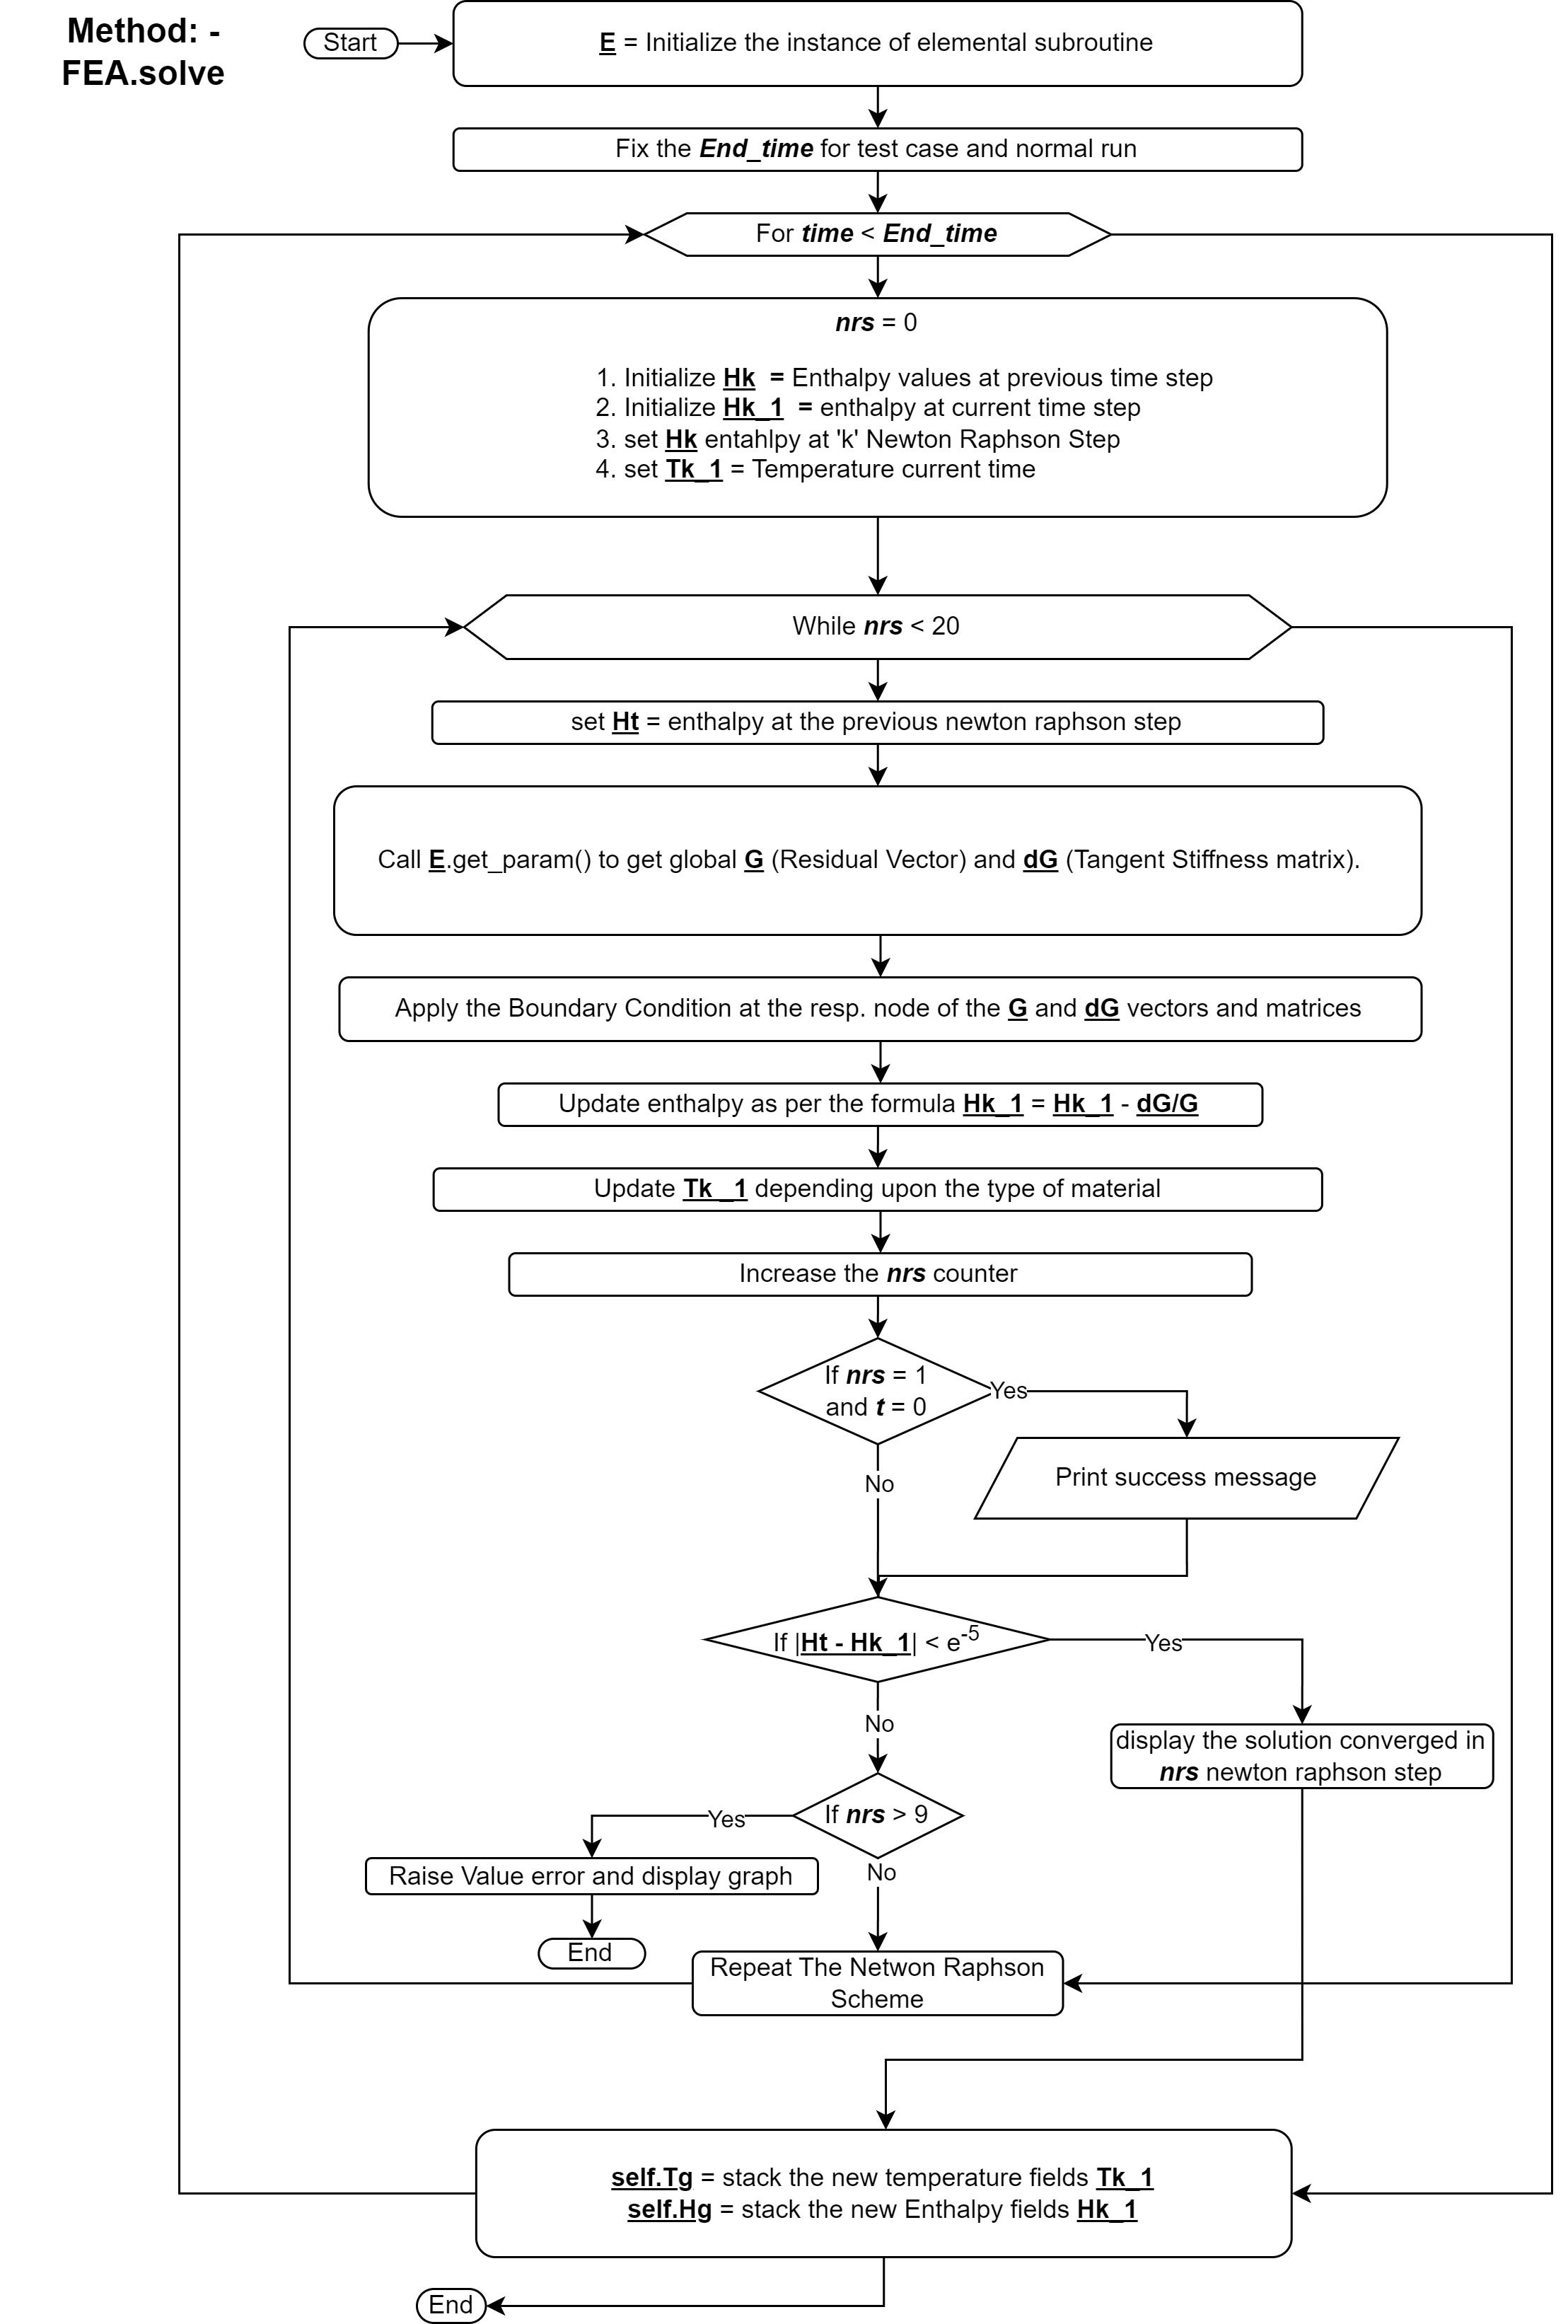
\includegraphics[width=13cm]{img/FEA_Solve.png}\\
  \caption{Main Class FEA}
  \label{fig:FEA_Solve}
\end{figure}

\begin{figure}[htb]
  \centering
  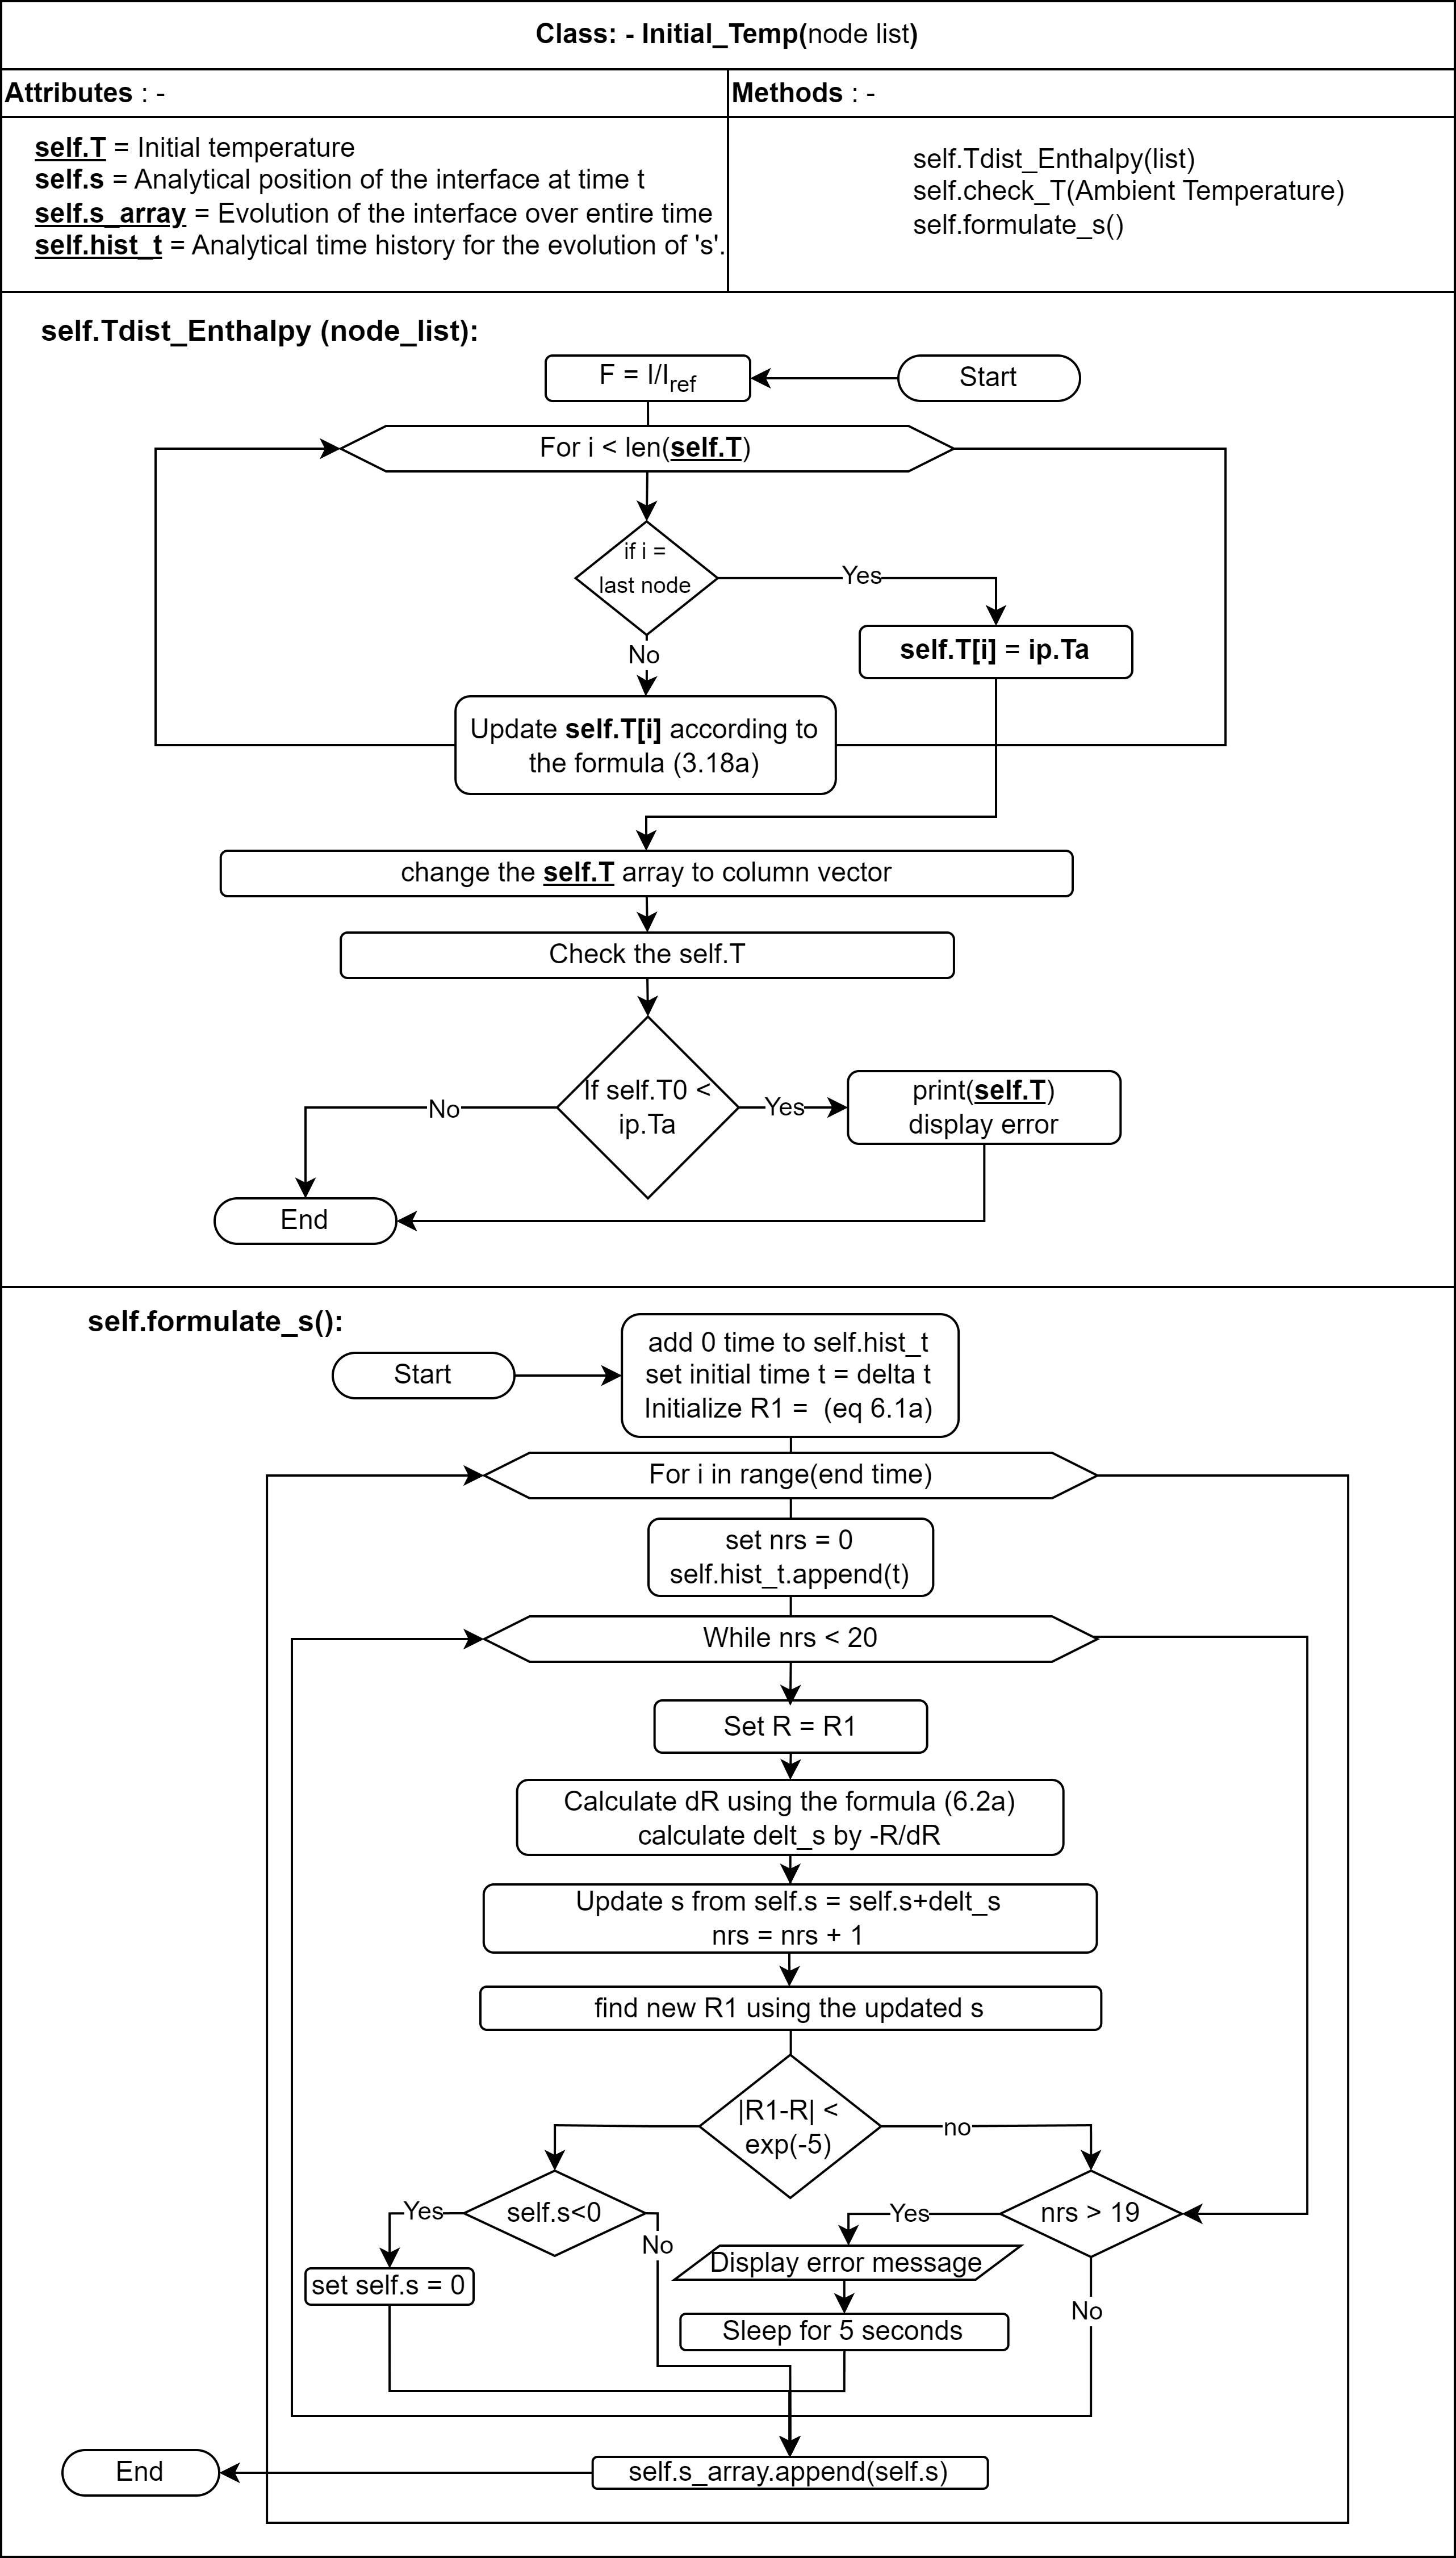
\includegraphics[width=11cm]{img/drawio.png}\\
  \caption{Class Initial Conditions}
  \label{fig:Initial Conditions}
\end{figure}

\begin{figure}[htb]
  \centering
  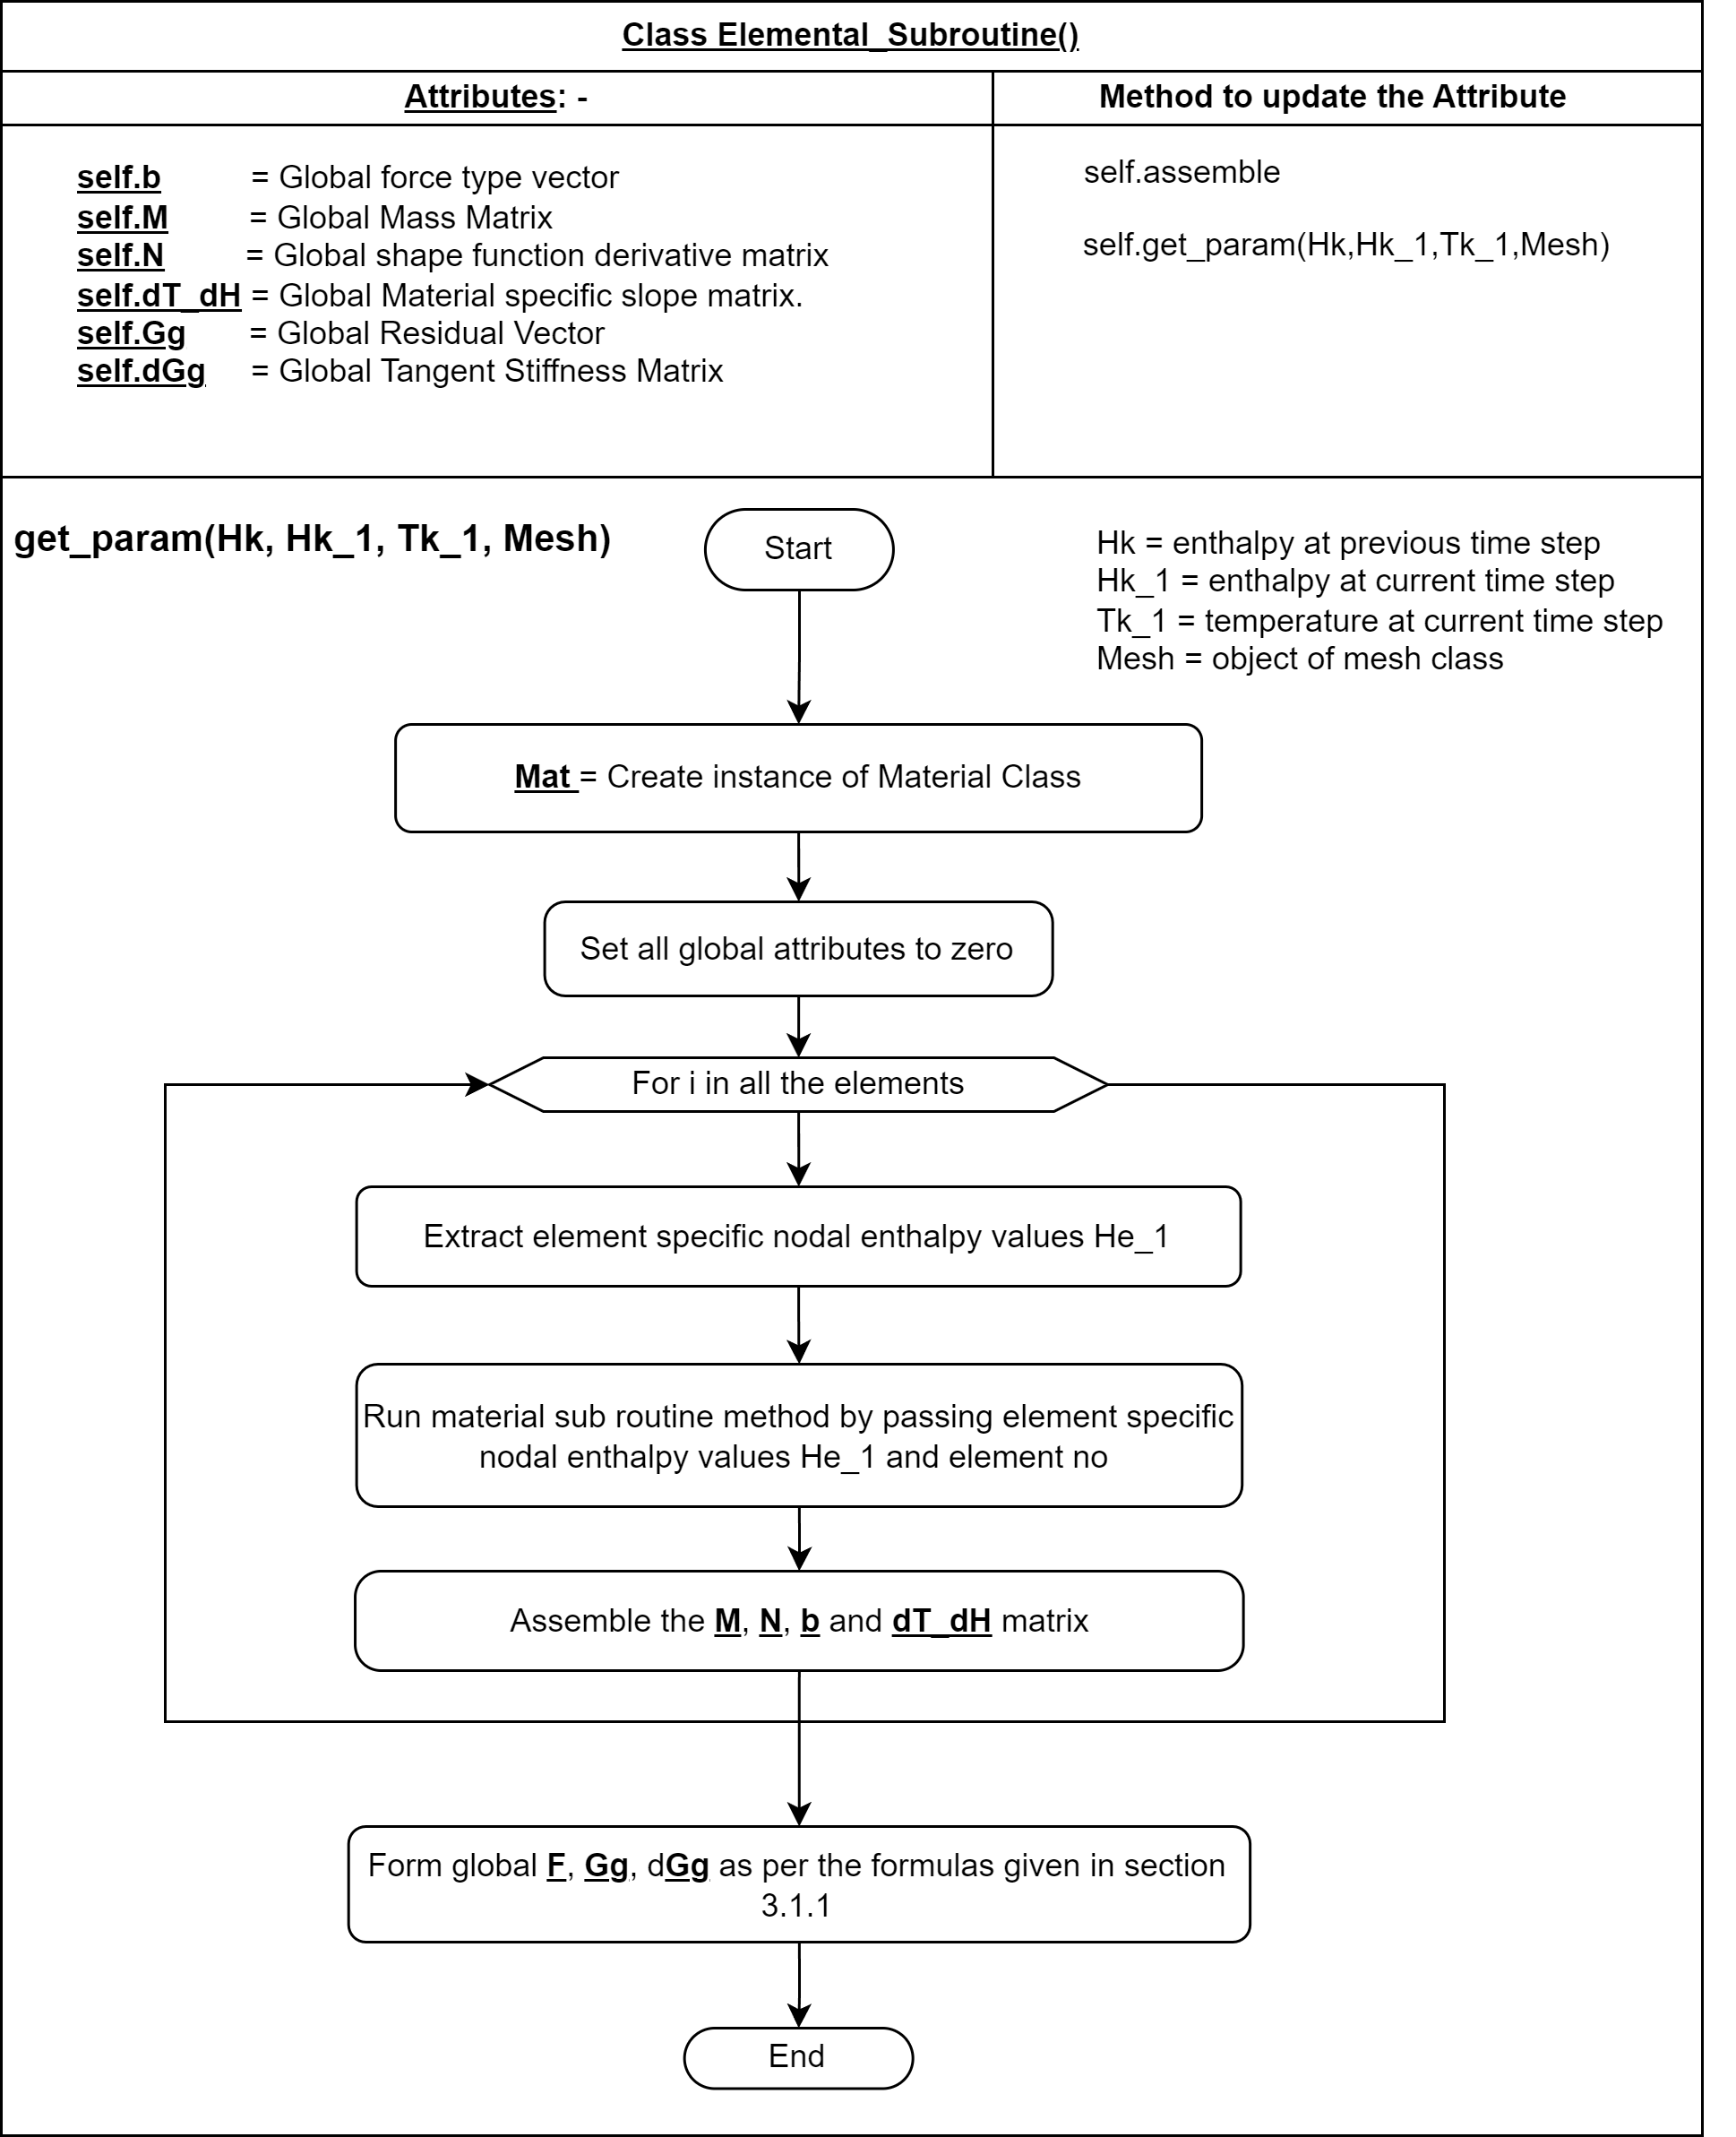
\includegraphics[width=13cm]{img/ElementalSubroution.drawio.png}\\
  \caption{Class Elemental Subroutine}
  \label{fig:Elemental Subroution}
\end{figure}
\begin{figure}[htb]
  \centering
  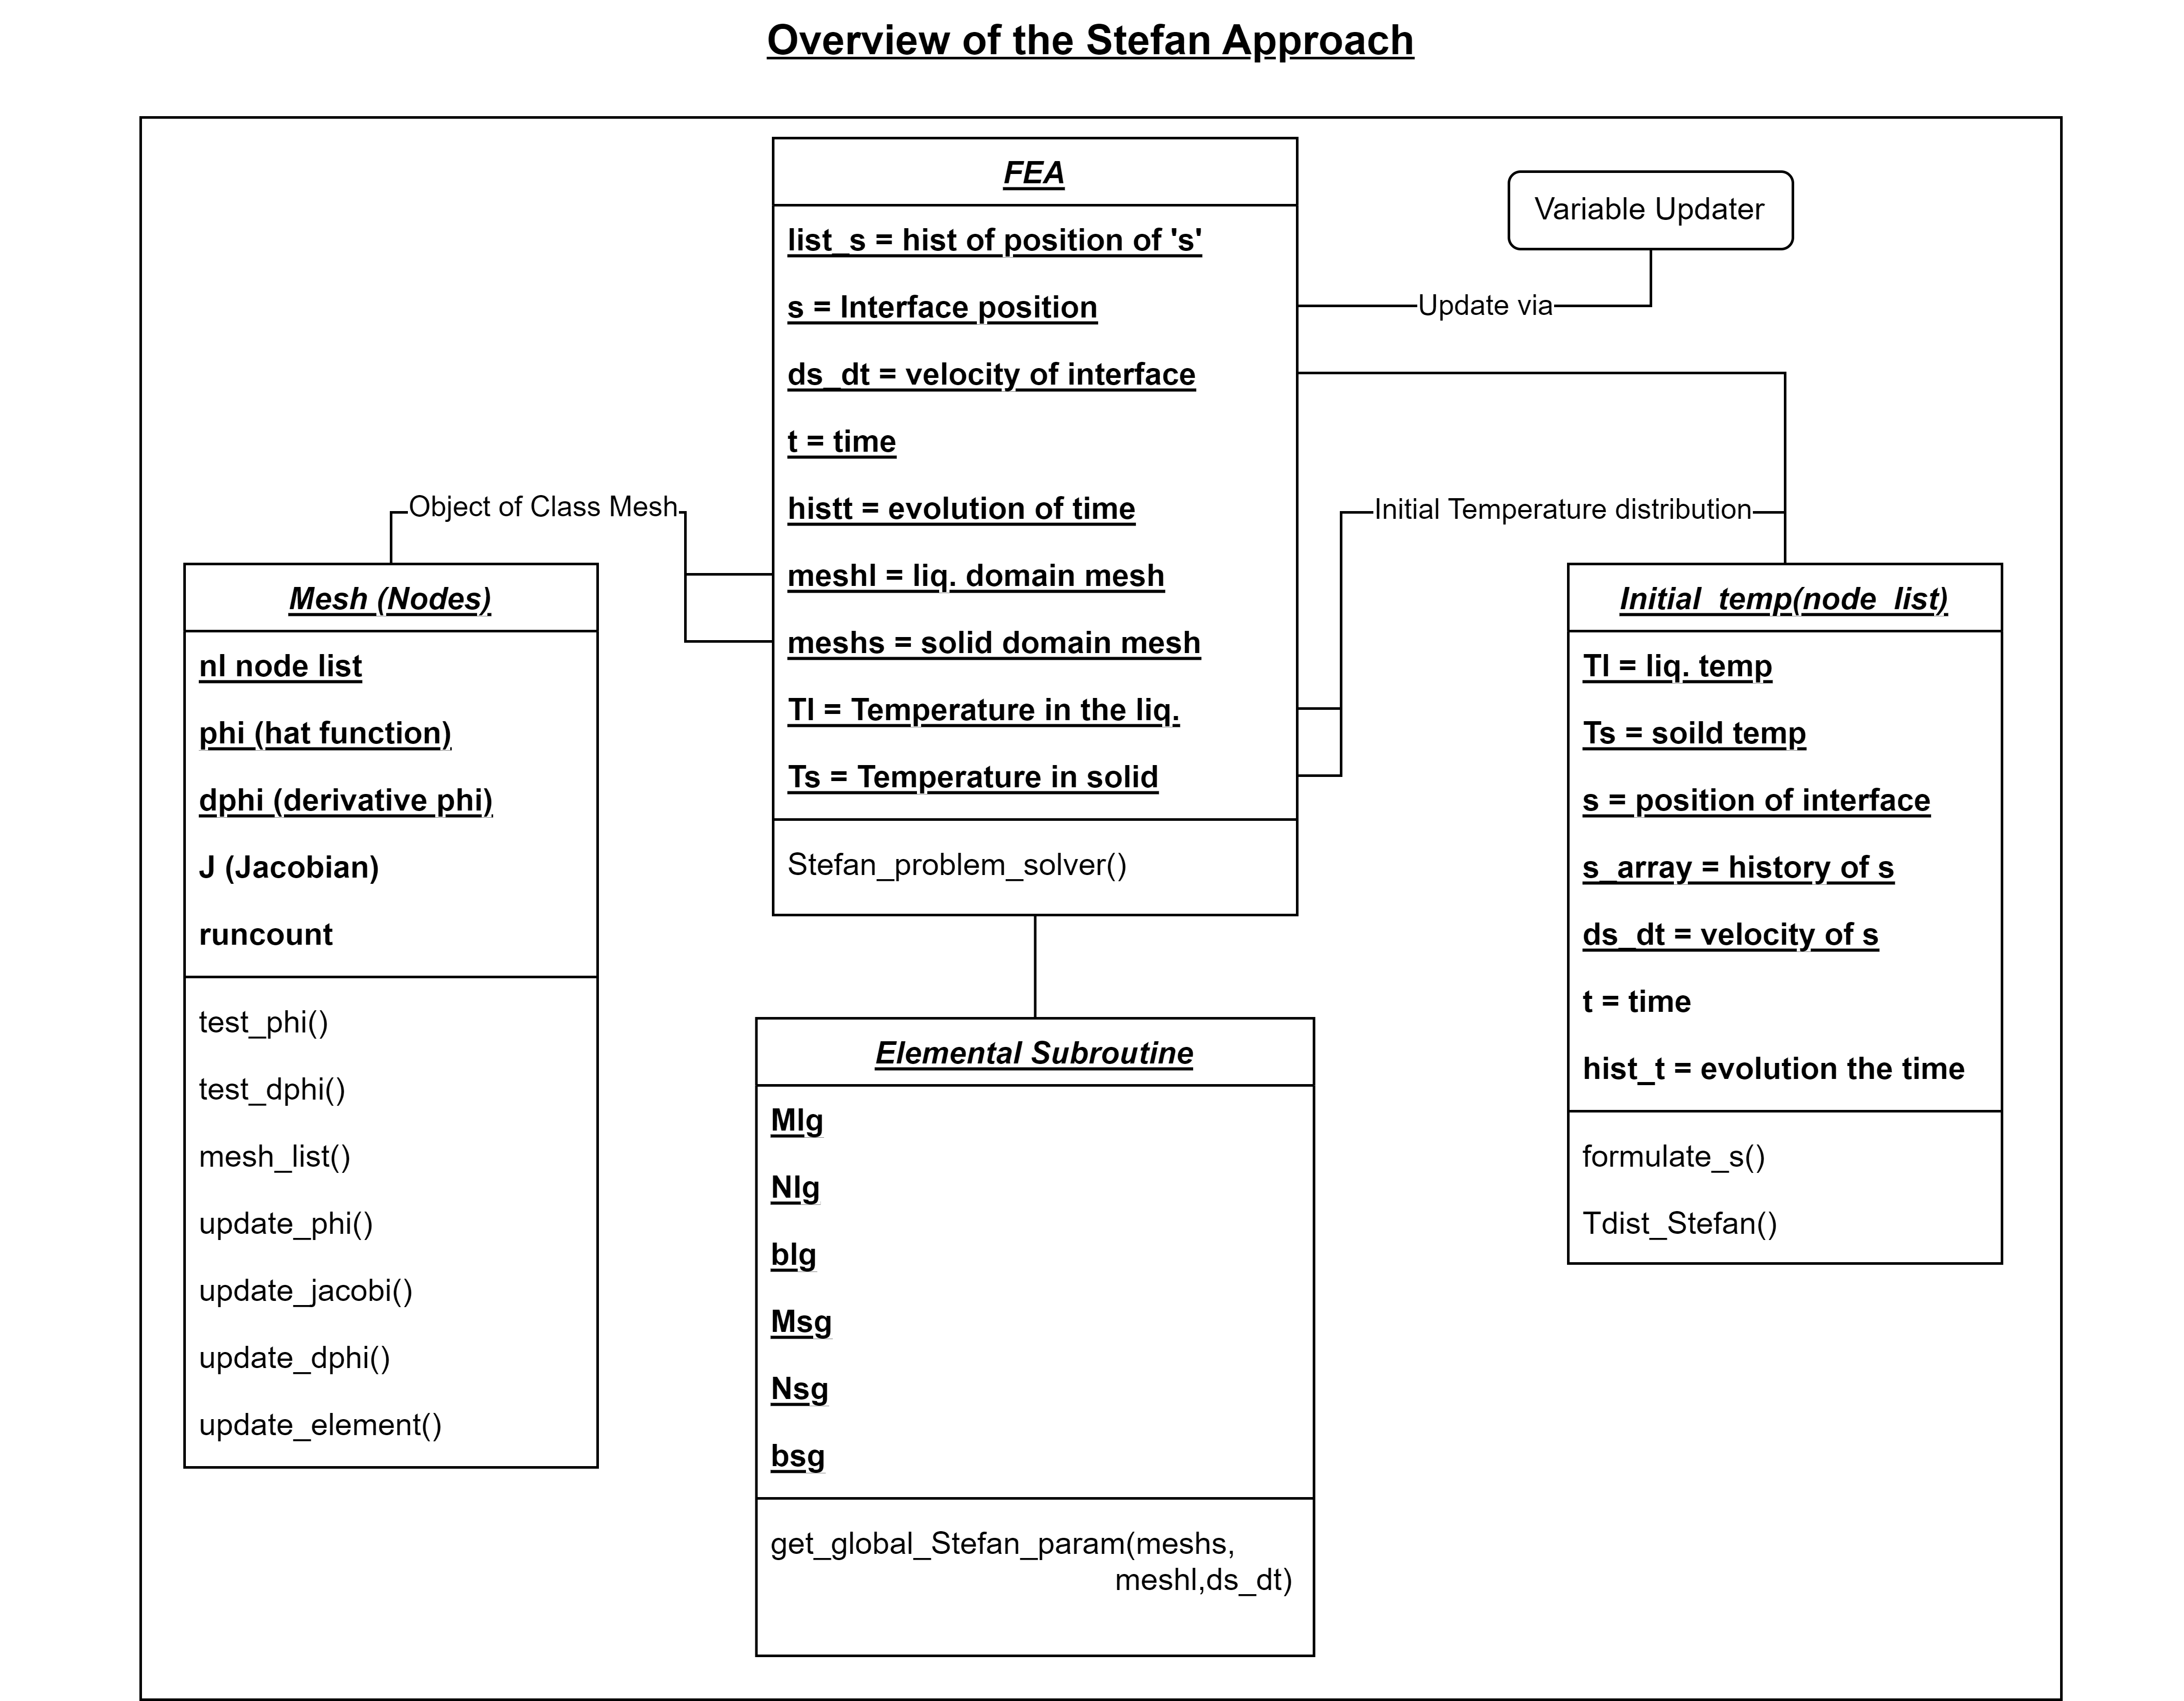
\includegraphics[width=13cm]{img/Stefan_Overview.png}\\
  \caption{Overview of the Stefan Problem Approach}
  \label{fig:overview Stefan Subroution}
\end{figure}
\begin{figure}[htb]
  \centering
  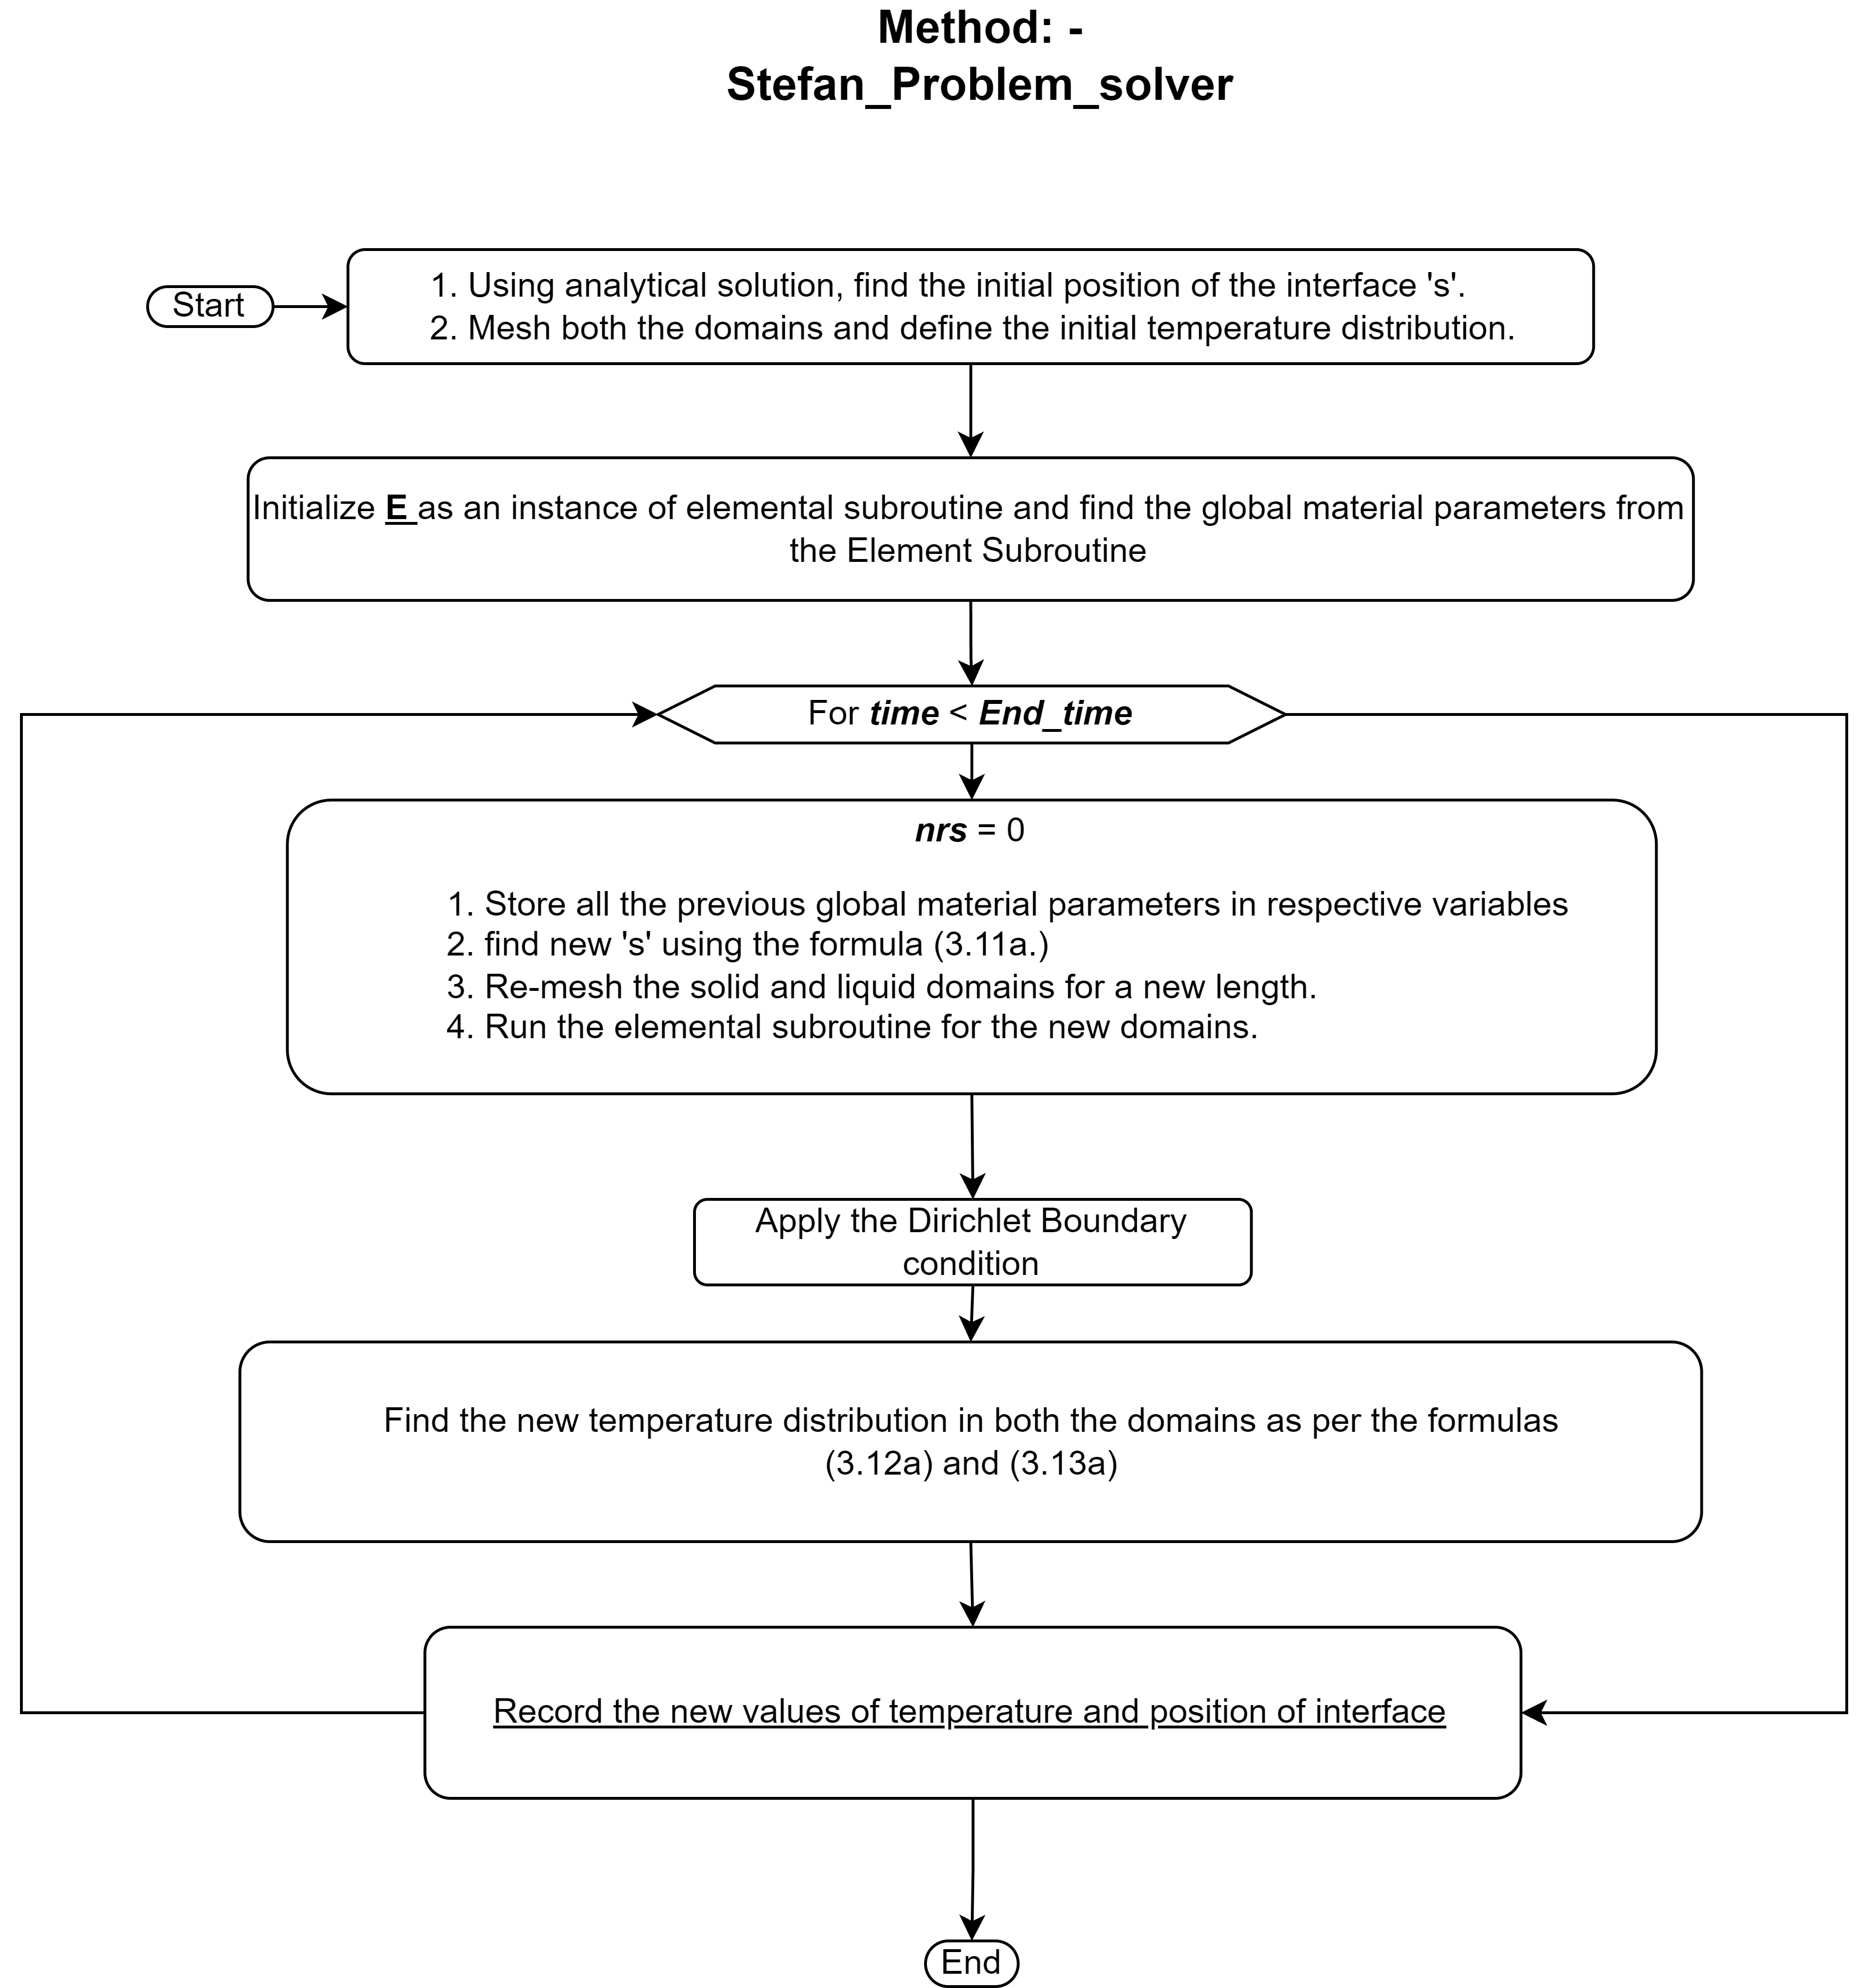
\includegraphics[width=13cm]{img/Stefan_Problem.png}\\
  \caption{Stefan Problem Solver}
  \label{fig:Stefan Problem Solver}
\end{figure}
